\begin{frame}{Conclusions and plans}
    \begin{tikzpicture}[overlay, remember picture]
        \node at (current page.center) {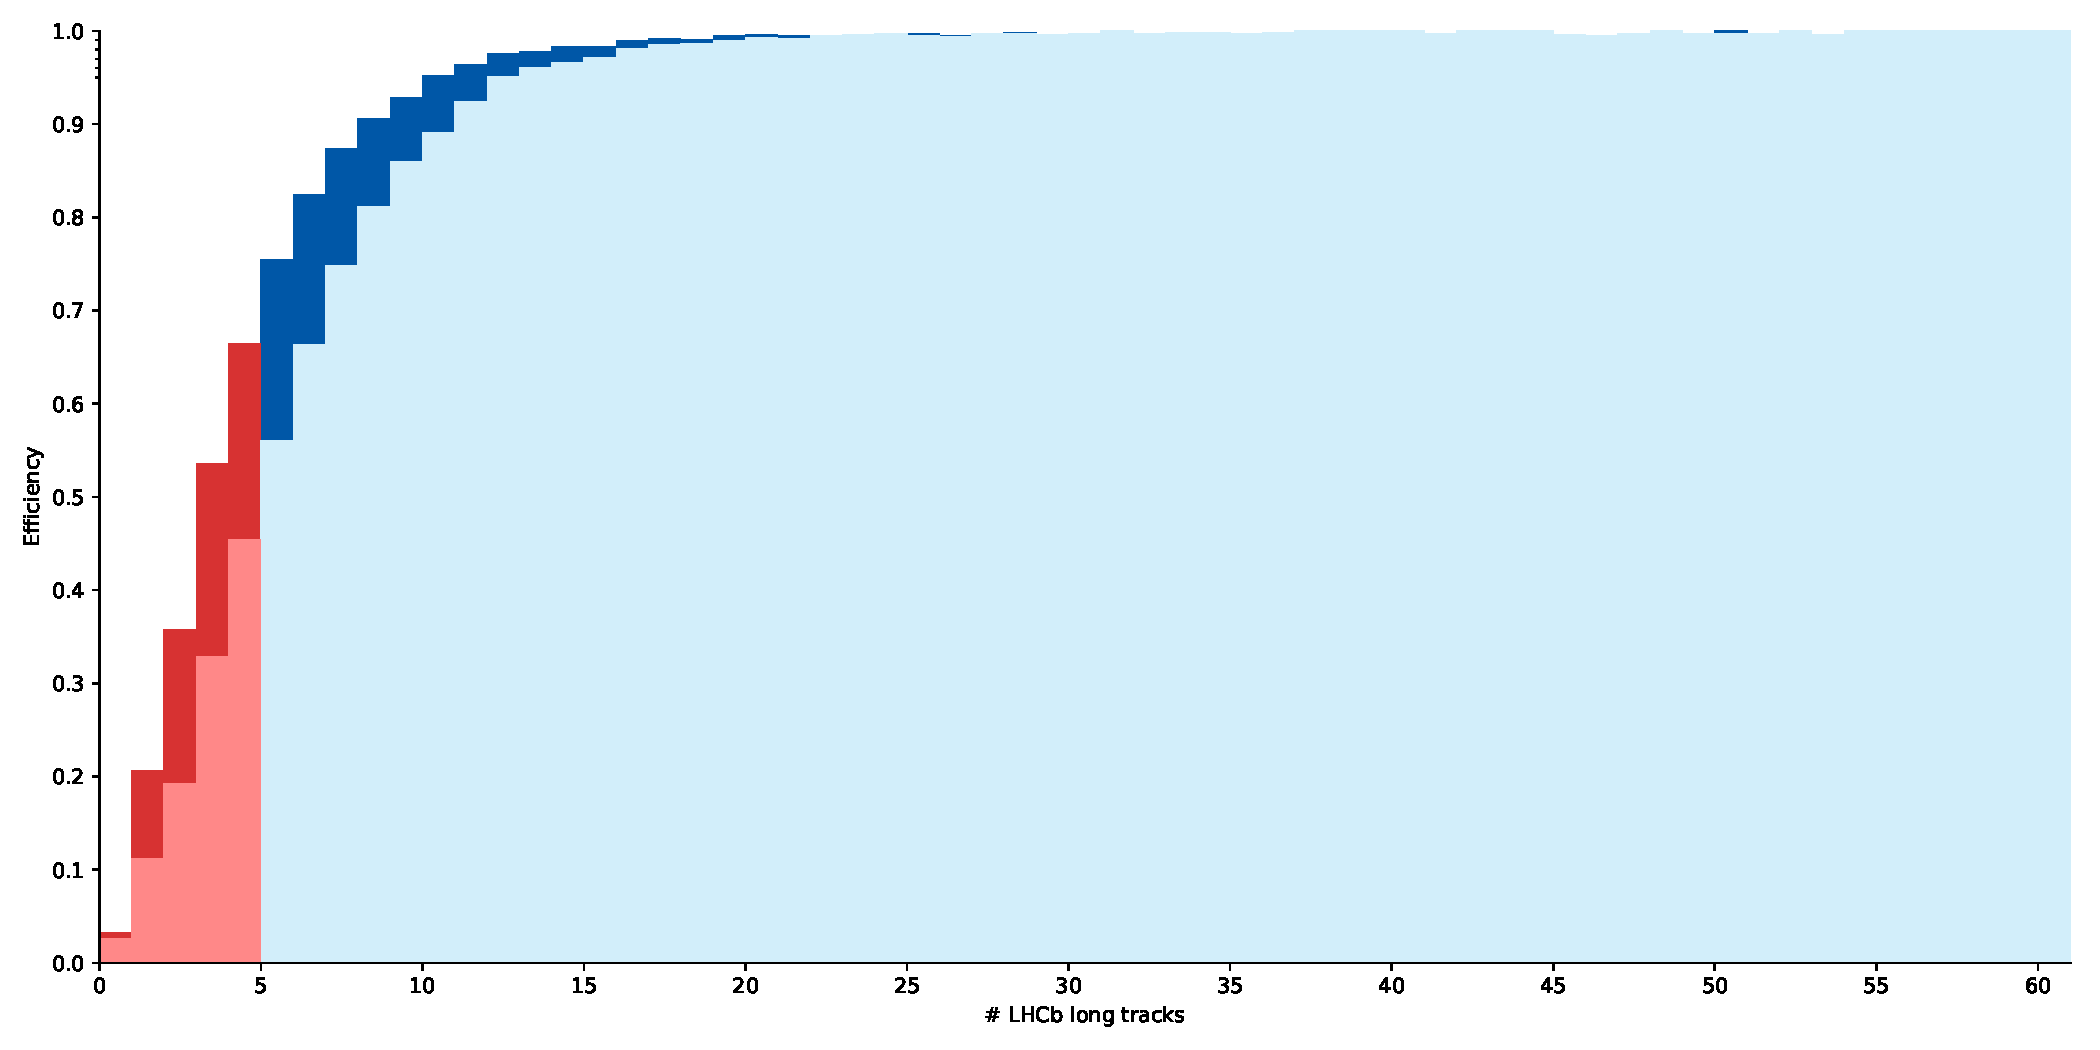
\includegraphics[width=14.7cm]{images/effntracks_bg.pdf}};
    \end{tikzpicture}
\begin{columns}
\column{.25\textwidth}
\column{.65\textwidth}
\setstretch{0.92}
\vskip -1.75em
    \begin{itemize}
    \setlength\itemsep{0.25em}
        \item [\textcolor{lhcbRed}{\textbullet}] \color{lhcbRed}
          Proof-of-Principle established:
          \color{lhcbBlue}
          a hybrid ML algorithm using a 1-dimensional KDE processed by a 5-layer CNN finds primary vertices with efficiencies and false positive rates similar to traditional algorithms.
        \item [\textcolor{lhcbRed}{\textbullet}] \color{lhcbRed} Efficiency is tunable; \color{lhcbBlue} increasing the efficiency also increases the false positive rate.
        \item [\textcolor{lhcbRed}{\textbullet}] \color{lhcbRed} Adding information
        should improve performance.
        \color{lhcbBlue}
        \begin{itemize}
            \item [\textcolor{lhcbBlue}
            {\textbullet} \color{lhcbBlue}] \color{lhcbBlue}
            can add KDE (x,y) information to algorithm
            \item [\color{lhcbBlue}{\textbullet} \color{lhcbBlue}]
            \color{lhcbBlue} can associate tracks to PV candidates, then iterate.
        \end{itemize}
        \item [\textcolor{lhcbRed}{\textbullet}] \color{lhcbRed} Next steps:
        \color{lhcbBlue}
        train with full LHCb MC and deploy inference engine in LHCb Hlt1 framework.
        \item [\textcolor{lhcbRed}{\textbullet}] \color{lhcbRed} Beyond LHCb
        \begin{itemize}
            \item [\color{lhcbBlue} {\textbullet}] \color{lhcbBlue}
            approach might work for ATLAS and CMS;
            \item [\color{lhcbBlue} {\textbullet}] \color{lhcbBlue} algorithm is an interesting ML laboratory.
        \end{itemize}
    \end{itemize}
\column{.1\textwidth}
\end{columns}
\end{frame}
